
\chapter{多视图几何基础}
\section{相机成像模型}


\section{相似变换、仿射变换、射影变换的区别}
\textbf{相似变换}。就是在刚体变换的基础上加了一个尺度因子,刚体变换是保距离和角度的变换,那么相似变换不保距离,但是保角度,保平行。

\textbf{仿射变换}。不保角度,保平行

\textbf{射影变换}。






\section{各种矩阵的区别}


单应矩阵,9个元素,因为相差一个尺度因子,所以自由度为8.那么为什么会相差一个尺度因子呢?因为单应矩阵变换时是作用在齐次坐标系下的,所以单应矩阵乘以一个任意非0的尺度因子,其得到的结果都是一样的。

基础矩阵,9个元素,因为相差一个尺度因子,并且基础矩阵的行列式为0(因为基础矩阵是奇异矩阵,为什么呢?因为基础矩阵1个点对应1条线,而不是1个点对应1个点),所以基础矩阵的的自由度为7。

本质矩阵,9个元素,5个自由度,旋转具有3个自由度,平移矩阵2个自由度(本来平移矩阵3个自由度,但是本质矩阵相差一个尺度因子),所以变成了两个自由度。


\section{单应矩阵和基础矩阵的应用场景}

单目相机进行初始化时,如果场景是平面、近似平面或低视差(low parallax)的场景,那么需要用\textbf{单应矩阵}进行初始化,非平面场景且视差足够大的情况下,需要使用\textbf{基础矩阵}进行初始化。

需要搞清楚为什么,就需要解决如下的两个问题:
\begin{enumerate}
	\item 为什么基础矩阵不能应用于平面场景
	\item 为什么单应矩阵不能应用于非平面场景。
\end{enumerate}


下面将依次介绍\textbf{纯旋转下单应矩阵和基础矩阵的区别},\textbf{平面场景下的基础矩阵}和\textbf{非平面场景下的单应矩阵}。

\subsection{纯旋转下的单应矩阵和基础矩阵}

基础矩阵的计算公式如下:
\begin{equation}
	F = K^T[t]_x RK
\end{equation}
可以看出,纯旋转的情况下,基础矩阵会挂掉,因为平移是0。所以纯旋转的情况下,不能够使用基础矩阵。或者从另一个方面来认知,对极几何必须要相机光心之间的基线不为零才有的,因此在纯旋转平移为零的情况下,自然是没有对极几何存在的,也就不能使用基础矩阵了。



在已知旋转和平移的情况下,单应矩阵的计算公式如下:
\begin{equation}
	H = R - tn^T/d
\end{equation}


在纯旋转$t = 0$的情况下, 可以发现矩阵$H$和深度$d$没有关系了,无论三维点是否在一个平面上,矩阵$H$都能符合它们之间的转换关系。又或者可以这样思考,每个3D点都在一个平面上(不同的3D点可以在相同或不同的平面上),平面通过$n$和$d$参数化,将其带入到公式中,由于在纯旋转的情况下,不管$n$和$d$是什么,求出来的单应矩阵$H$都是一样的,所以纯旋转的情况下能够使用单应矩阵。





\subsection{平面场景下的基础矩阵}


\textbf{为什么基础矩阵不能应用于非平面场景}。基础矩阵的计算公式如下:
\begin{equation}
	F = K^T[t]_x RK
\end{equation}
可以看出,纯旋转的情况下,基础矩阵会挂掉,因为平移是0,不过这不是重点。下面来推导为什么基础矩阵不能用于平面场景。假设场景是平面且能够使用基础矩阵,那么就有如下两个公式:
\begin{equation}
	x' = Hx
\end{equation}
\begin{equation}
	x^TFx' = 0
\end{equation}

将$x' = Hx$带入到公式$x^TFx'=0$中,得到:
\begin{equation}
	x'FHx = 0
\end{equation}
可以看到这个一个二次型,二次型为0,那么二次型矩阵是反对称矩阵,也就是说只要矩阵$FH$是一个反对称矩阵,这个等式就永远成立,也就是说求得的基础矩阵并不唯一(这可不是尺度不确定的那种不唯一)。并且反对称矩阵只有3个自由度,

\begin{note}
但是这也只能说明$FH$只有3个自由度,而不能说明$F$只有3个自由度,也不能说明基础矩阵$F$退化啊。
\end{note}


下面是另一种推导,表示本质矩阵和基础矩阵在平面情况下会产生退化,从而导致有无穷多个解满足情况。
\begin{equation}
	x' = Hx
\end{equation}
我们知道一个向量和自己叉乘的结果为零向量,所以有
\begin{equation}
	\hat{x}‘x’ = 0 \rightarrow \hat{x}‘Hx = 0
\end{equation}

另外,任意不与$x'$平行的三维向量$u$和$x'$的叉乘结果垂直于向量$x'$(叉乘的物理意义),所以有:


\begin{equation}
\begin{split}
\hat{u}x' & \perp Hx \\
 \Rightarrow &  (\hat{u}x')^THx = 0 \\
 \Rightarrow & -x'^T\hat{u}Hx1 = 0 \\
 \Rightarrow & x'^T\hat{u}Hx = 0
\end{split}
\end{equation}


所以我们能够得到$E=\hat{u}E$,这说明$E$在这种情况下有无穷多解都能满足$x'^TEx = 0$,由于$F=K^TEK$,所以也说明$F$有无穷多解。所以说在平面情况下,求解基础矩阵会发生退化。

\begin{note}
你可能会觉得,只要给定的对应点$x'$和$x$的数量足够多,那么就能够减少矩阵$E$或$F$的的解的个数。但是三维空间中肯定存在任意多个向量$u$不与给定的所有向量$x'$平行,也就是说仍旧有无穷多个$E$满足情况。
\end{note}




\subsection{非平面场景下的单应矩阵}
单应矩阵的公式如下:
\begin{equation}
	H = R - tn^T / d
\end{equation}

假设场景是非平面的,然后我们通过RANSAC算法估计了一个满足大多数点对应情况的单应矩阵。那么也就是说我们拟合了一个潜在的平面(其参数为$n$和$d$),如图\ref{fig:nonplanar_homography}所示。所以我的理解是,在使用RANSAC+DLT方法计算单应矩阵时(随机选择4个点),就相当于隐式地计算了潜在平面的参数$n$和$d$。然后在计算内点时,就是要找到误差比较小的点,那么理论上应该是那些距离潜在平面比较近的点,因为对应那些不在平面上的3D点所对应的2D点(左图像上的点),利用单应矩阵转换之后,会强迫其落在潜在平面上,然后再投影到右平面上。这个过程中,离平面近的点产生的误差比较小,而离平面较远的点产生的误差比较大。所以在使用RANSAC+DLT算法求解单应矩阵时,应该就是在3D空间中找到一个平面,使得该平面周围的点尽可能多。


所以说,在非平面场景下使用单应矩阵时,如果特征点所对应的3D点中存在这样一个满足大多数点的平面,那么求得的单应矩阵所对应的内点就多,否则内点数就少。

\begin{note}
	以上的推导纯粹我自己的理解,并不一定正确,因为推导的使用并没有将旋转平移也考虑在内。而且我的这个推导并不能解决\textbf{低视差}情况下能够使用单应矩阵。
\end{note}

\begin{figure}[h]%%图
	\centering  %插入的图片居中表示
	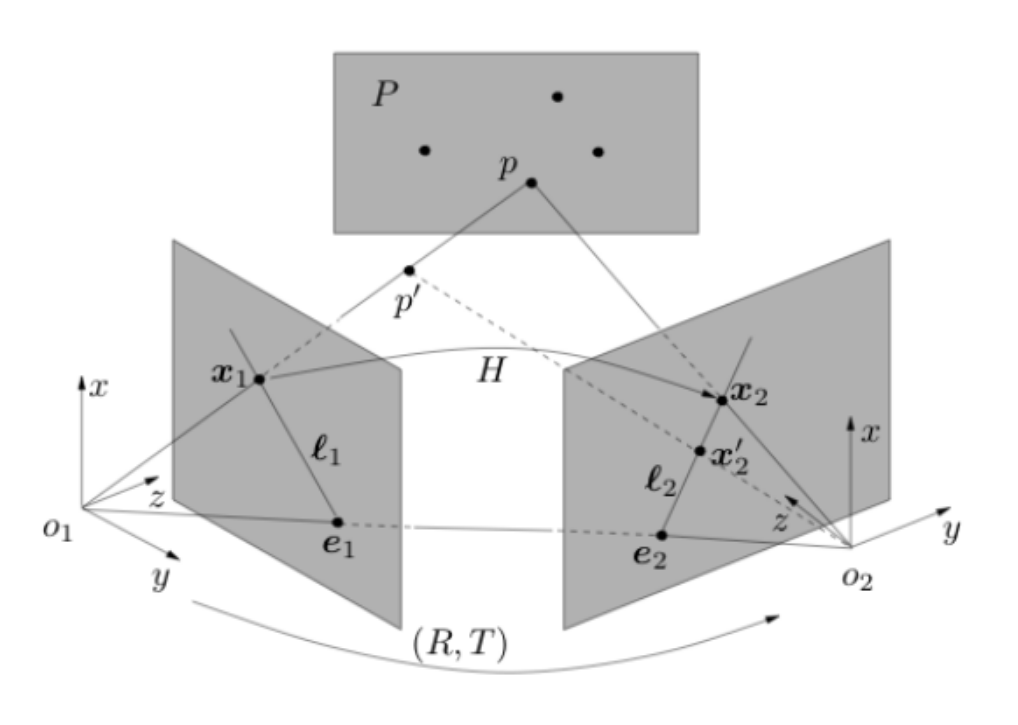
\includegraphics[width=0.6\linewidth]{image/Multiview-Geometry-Base/nonplanar_homography.png}  %插入的图,包括JPG,PNG,PDF,EPS等,放在源文件目录下
	\caption{非平面场景下的单应矩阵.}  %图片的名称
	\label{fig:nonplanar_homography}   %标签,用作引用
\end{figure}



\section{各种矩阵计算}

\subsection{单应矩阵求解}
单应矩阵,DLT

归一化方法
\subsection{基础矩阵求解}
基础矩阵,8点法,7点法
\subsection{本质矩阵求解}

本质矩阵,8点法,5点法

\section{位姿计算}
\subsection{2D-2D,分解本质矩阵}
4个解
\subsection{2D-2D,分解单应矩阵}
8个解



\subsection{2D-3D}

PnP问题的求解方法归纳如下:
~\\ % 插入空行

\begin{tabular}{|c|c|c|c|c|}
	\hline
	PnP方法 & 是否需要内参K & 需要的2D-3D对应点数 & 精度 & 速度 \\
	\hline
	DLT & No & 6 & Medium & Fast   \\
	P3P& Yes & 3(4)& Medium & Fast \\
	EPnP(Efficient PnP)Yes & 4 & High & Fast   \\
	UPnP & No & 4 & Medium & Fast  \\
	MRE(LSI,最小二乘迭代) & Yes & 3 & Highest & Slow \\
	\hline
\end{tabular}

~\\

\textbf{DLT}。DLT方法就像DLT放方法求解单应矩阵一样,直接将R和t看做是未知变量,那么可知道有12个未知变量,而每个2D-3D点对应可以给定两个方程。所以只需要6个点构成12个方程就能够求解R和t。但是DLT求解时,忽略了元素的内在关系,对于t的求解没有什么问题,但是求解出来的旋转矩阵R可能并不满足旋转矩阵的性质,旋转矩阵是正交矩阵且行列式为1。解决方法就是求解一个最好的旋转矩阵对其进行近似,这可以由QR分解(将矩阵分解成正交矩阵Q和上三角矩阵R)完成。
\begin{note}
	QR分解中的Q就是我们要的旋转矩阵吗?如果内参未知,那么也能够通过DLT方法求解,那么此时需要几个点对应来进行求解呢?
\end{note}


\textbf{P3P}。P3P算法的思想在于,求得3个3D点(世界坐标系)在当前相机坐标系下的坐标,那么就得到了3对3D-3D点对应,从而将问题转为3D-3D的位姿估计问题,因为\textbf{带有匹配信息}的3D-3D位姿求解非常容易。P3P算法利用3对点求解位姿后,会得到4个解,因此还需要一对额外的点来验证4个解中哪个解是正确的。


\textbf{EPnP}。其思想也是将2D-3D求位姿问题,转化为3D-3D求位姿问题。不过EPnP把问题转为了世界坐标系下和当前坐标系下4对3D控制点的位姿求解问题。只要搞懂了如何求解两个坐标系下的控制点的坐标,那么就将EPnP算法给搞懂了。

\textbf{UPnP}。

\textbf{LSI}。这种方法求解位姿就是将位姿求解问题构造成一个优化问题,通过将损失函数构造位重投影误差,待优化变量为在李代数上的se3,通过最小化该误差从而求解位姿。由于是迭代方法,所以该方法需要给定一个初始位姿。ORB-SLAM2就用了这种方法来追踪下一帧图像的位姿。



\begin{note}
	既然LSI方法的精度高,那么是不是可以在用其它方法求得一个位姿后,再用LSI对该解进行迭代求精。可以用在我的SFM程序里面提高效果。
\end{note}


\subsection{3D-3D}

通过3D-3D对应求解位姿的方法分两种,一种是通过SVD矩阵分解的方式,另一种则是通过迭代优化误差的方法。

一般来说,通过3D-3D求位姿,使用的都是ICP算法及其变种。例如,对齐两个用激光雷达扫描得到的点云就需要使用ICP算法。不过在视觉SLAM中,3D-3D点对应之间的匹配关系是知道的,这大大降低了问题的难度。

\textbf{SVD方法}。


\textbf{迭代方法}。通过将旋转和平移构造成误差函数,待优化变量为李代数上的se3,通过最小化该误差从而求解位姿。《视觉SLAM14讲》中说ICP问题存在唯一解或无穷多解的情况,在唯一解的情况下,只要我们找到了极小值解,那么\textbf{这个极小值解就是全局最优值}。这意味着ICP求解可以任意选定初始位姿,\textbf{这是已知匹配点时求解ICP问题的一大好处}。

\begin{note}
	至于什么时候存在唯一解,什么时候存在无穷多解,《视觉SLAM14讲》让我们去看《State estimation for robotics : A matrix lie group approach》
\end{note}


\section{三角测量}




\section{参考文献}
透镜畸变及校正模型
https://blog.csdn.net/dcrmg/article/details/52950141


图像矫正去畸变
https://blog.csdn.net/weixin\_38009585/article/details/82356022


A Review of Solutions for Perspective-n-Point Problem in Camera Pose Estimation
https://iopscience.iop.org/article/10.1088/1742-6596/1087/5/052009/pdf


相机位姿求解——P3P问题
https://www.cnblogs.com/mafuqiang/p/8302663.html

epnp算法简介
https://blog.csdn.net/eric\_e/article/details/80953100

深入EPnP算法
https://blog.csdn.net/jessecw79/article/details/82945918

SVD求解3D-3D位姿估计
https://zhuanlan.zhihu.com/p/51362089


相机位姿求解问题?
https://www.zhihu.com/question/51510464/answer/132005467



